\documentclass[11pt,letterpaper]{article}
\usepackage[margin=1in]{geometry}
\usepackage[english]{babel}
\usepackage[utf8x]{inputenc}
\usepackage{amsmath}
\usepackage{amssymb} 
\usepackage{graphicx}
\usepackage{tabularx}
\usepackage{epstopdf}
\usepackage{subfig}
\usepackage{bbm}
\usepackage{kpfonts}    % for nice fonts
\usepackage{microtype} 
\usepackage{booktabs}   % for nice tables
\usepackage{bm}         % for bold math
\usepackage{listings}   % for inserting code
\usepackage{verbatim}   % useful for program listings
\usepackage{color}  
\usepackage[colorlinks=true]{hyperref}
\usepackage{setspace}
% use for hypertext

\usepackage{natbib}
\usepackage{authblk}
\usepackage[hang,flushmargin,multiple]{footmisc} %dont indent footnotes
\newcommand{\hilight}[1]{\colorbox{yellow}{#1}}
\hypersetup{colorlinks=true,linkcolor=black,citecolor=black,urlcolor=black}

\newcolumntype{K}[1]{>{\centering\arraybackslash}p{#1}}



\title{Benefits in a SNAP: The Effects of the Online Food Stamps Application Rollout}
\author{Andrew Foote and Michel Grosz and}
\date{\today\\  }





\begin{document}
\maketitle

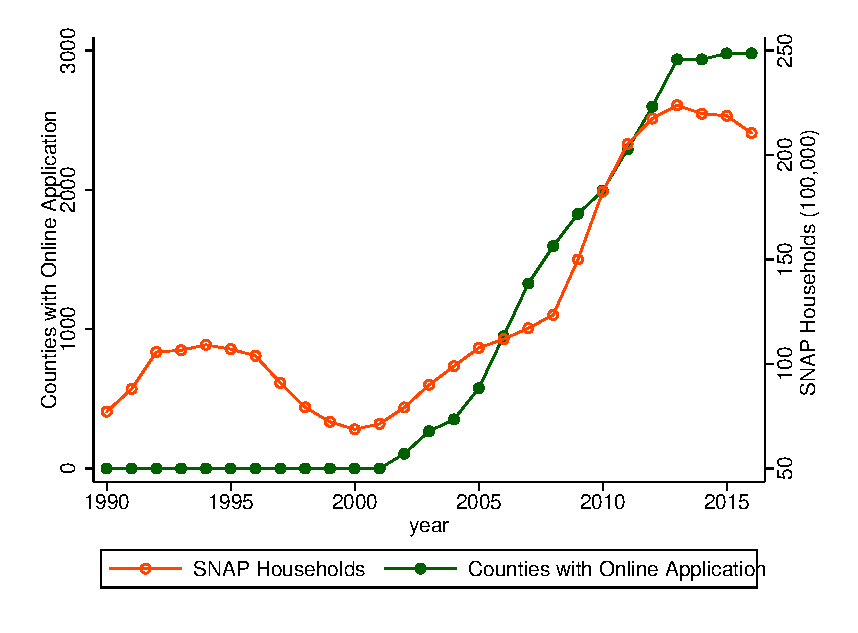
\includegraphics{rolloutgraph}

\begin{figure}\caption{Event Study Estimates}
\begin{tabular}{cc}
\includegraphics[scale=0.57]{evstu_notr_5_3}&\includegraphics[scale=0.57]{evstu_sttr_5_3}\\
a) County Fixed Effects&b) County Fixed Effects and State Trends\\
\includegraphics[scale=0.57]{evstu_cttr_5_3}\\c) County Fixed Effects and County Trends\\
\end{tabular}
\end{figure}
\end{document}
